%
% The first command in your LaTeX source must be the \documentclass command.
% \documentclass[acmtog]{acmart}
\documentclass[sigchi]{acmart}
\settopmatter{printacmref=false}
\settopmatter{printacmref=false}
\setcopyright{none}
\settopmatter{printacmref=false} % Removes citation information below abstract
\renewcommand\footnotetextcopyrightpermission[1]{} % removes footnote with conference information in first column
\pagestyle{plain} % removes running headers
\renewcommand\footnotetextcopyrightpermission[1]{}

\usepackage{color}
\usepackage[usenames,dvipsnames,svgnames,table]{xcolor}
%
% defining the \BibTeX command - from Oren Patashnik's original BibTeX documentation.
% \def\BibTeX{{\rm B\kern-.05em{\sc i\kern-.025em b}\kern-.08emT\kern-.1667em\lower.7ex\hbox{E}\kern-.125emX}}
%
% The majority of ACM publications use numbered citations and references. If you are preparing content for an event
% sponsored by ACM SIGGRAPH, you must use the "author year" style of citations and references. Uncommenting
% the next command will enable that style.
%\citestyle{acmauthoryear}
%
% end of the preamble, start of the body of the document source.

\begin{document}

%
% The "title" command has an optional parameter, allowing the author to define a "short title" to be used in page headers.
\title{    
	Project 3: Continuous Control\\
	{\large Udacity Deep Reinforcement Learning Nanodegree Program}
}

%
% The "author" command and its associated commands are used to define the authors and their affiliations.
% Of note is the shared affiliation of the first two authors, and the "authornote" and "authornotemark" commands
% used to denote shared contribution to the research.
\author{Bob Flagg}\affiliation{}

%
% By default, the full list of authors will be used in the page headers. Often, this list is too long, and will overlap
% other information printed in the page headers. This command allows the author to define a more concise list
% of authors' names for this purpose.
\renewcommand{\shortauthors}{Bob Flagg}

%
% The abstract is a short summary of the work to be presented in the article.

%
% The code below is generated by the tool at http://dl.acm.org/ccs.cfm.
% Please copy and paste the code instead of the example below.
%

%
% A "teaser" image appears between the author and affiliation information and the body 
% of the document, and typically spans the page. 
\begin{teaserfigure}
	\centering
  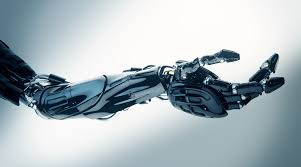
\includegraphics[width=0.4\textwidth]{arm}
  \caption{Designing a robotic arm. Source: SOLIDWORKS 2016}
  \label{fig:teaser}
\end{teaserfigure}

%
% This command processes the author and affiliation and title information and builds
% the first part of the formatted document.
\maketitle

%%%%%%%%%%%%%%%%%%%%%%%%%%%%%%%%%%%%%%%%%%%%%%%%%%%%%%%%%%%%%%
%% Introduction                                                                                                                             %%
%%%%%%%%%%%%%%%%%%%%%%%%%%%%%%%%%%%%%%%%%%%%%%%%%%%%%%%%%%%%%%
\section{Introduction}

In this project I'll implement a solution to the 
\href{https://github.com/Unity-Technologies/ml-agents/blob/master/docs/Learning-Environment-Examples.md#reacher}{\underline{Reacher}}
environment from the 
\href{https://unity3d.ai}{\underline{Unity Machine Learning Toolkit}}.
The Reacher is a double-jointed arm that can move to target locations. A reward of +0.1 is provided for each step 
that the agent's hand is in the goal location. Thus, the goal for the agent is to maintain its position at the target location for as many time steps as possible.

The observation space consists of 33 variables corresponding to position, rotation, velocity, and angular velocities of the arm. Each action is a vector with four numbers, corresponding to torque applicable to two joints. Every entry in the action vector should be a number between -1 and 1.


I'll use {\em Deep Deterministic Policy Gradient}~\cite{Silver:2014:DPG:3044805.3044850} (DDPG) to solve the distributed version of the task which contains 20 identical agents, each with its own copy of the environment.
Source code in Python, using PyTorch, is available on 
\href{http://github.com}{\underline{github}} 
in the repo 
\href{https://github.com/bobflagg/Continuous-Control}{\underline{Continuous-Control}}.





\section{Background}

The 
\href{https://github.com/Unity-Technologies/ml-agents/blob/master/docs/Learning-Environment-Examples.md#reacher}{\underline{Reacher}}
is a {\em sequential decision making problem}, in which an agent interacts with an environment over discrete time
steps and tries to find a {\em policy} to maximize the expected {\em discounted return}:
$$G_t = \sum_{k=0}^{\infty}\gamma^kR_{t+k+1},$$
where $\gamma\in[0,1]$  is a discount factor that trades-off the importance of immediate and future rewards.
See~\cite{DBLP:books/lib/SuttonB98} for a general discussion of this sort of problem. 

In this project I will use policy-based methods, which try to directly  find an {\em optimal policy}, $\pi^*$,  that an agent can use to decide what actions to take.  The
particular algorithm,
 {\em Deep Deterministic Policy Gradient}~\cite{Silver:2014:DPG:3044805.3044850} (DDPG),
is motivated by an important connection between the action selected by an optimal policy and the {\em optimal action-value function} 
	$$Q^*(s, a) =  \max_{\pi}Q^{\pi}(s,a).$$
Namely, if you know the optimal action-value function, then in any given state, $s$, an optimal action can be found by solving
	 $$\pi^*(s) = \arg\max_a Q^*(s,a).$$
 DDPG concurrently learns an approximator to $Q^*(s,a)$ and an approximator to $\pi^*(s)$, and it does so in a way which is specifically adapted for environments with continuous action spaces. 

\subsection{Learning $Q^*(s,a)$}

The starting point for approximating $Q^*(s, a)$  is the \textbf{Bellman Equation}:
$$Q^{*}(s,a) = \mathbb{E}\big[R_{t+1}+\gamma\cdot \max_{a'}Q^{*}(S_{t+1},a')| S_t = s, A_t=a\big].$$
Suppose we are approximating $Q^*(s, a)$ with a neural network, $Q_\phi(s,a)$, and we have collected a set $\mathcal{D}$ of
transitions $(s, a, r, s', d)$, then the \textbf{mean-squared Bellman error} (MSBE)
		$$L(\phi, \mathcal{D}) = \mathbb{E}_{\mathcal{D}}\big[\big(Q_\phi(s,a)-(r+\gamma\cdot(1-d)\max_{a'}Q_\phi(s',a'))\big)^2\big]$$
tells us roughly how closely $Q_{\phi}$ comes to satisfying the Bellman equation and so can serve as the loss function in tuning $\phi$.

\subsection{Learning $\pi^*(s)$}

Learning the optimal policy is pretty simple: we want to learn a deterministic policy $\pi^*(s)$ which gives the action that maximizes $Q^*(s, a)$.
For this DDPG uses a neural network, $\pi_\theta(s)$, and loss function
$$L(\theta, \mathcal{D}) = -\mathbb{E}_{\mathcal{D}}\big[Q_\phi(s,\pi_\theta(s))\big].$$
 

\section{DDPG for Continuous Control}

I've implemented DDPG for the \href{https://github.com/Unity-Technologies/ml-agents/blob/master/docs/Learning-Environment-Examples.md#reacher}{\underline{Reacher}}
in the notebook 
\href{https://nbviewer.jupyter.org/github/bobflagg/Continuous-Control/blob/master/01-Continuous-Control-with-DDPG.ipynb}{\underline{Continuous-Control-with-DDPG}}.
The key components and hyper-parameter settings are outlined below.
\begin{itemize}
	\item \textbf{Actor Network}: One fully connected linear hidden layer with 256 units. The input size is equal to the environment state-size and the output size is equal to the environment action-size. It uses ReLu activation functions and batch normalization after the hidden layer.
	\item \textbf{Critic Network}: Three fully connected linear hidden layers. The first hidden layer has 256 units and has input size equal to the environment state-size. The second hidden layer has 256 units and input size equal to 256 + the environment action-size. The third hidden layer has 128 units. ReLu activation functions are used throughout  and batch normalization is applied after the first layer. The output of this network is one-dimensional.
	\item \textbf{Hyperparameter Settings}: 
	I trained for 150 episodes with a batch size of 64, discount factor of $\gamma = 0.99$, soft update weight of $\tau = 0.001$, actor learning rate of $0.0001$, 
	 and critic learning rate of $0.001$.  To get DDPG to learn in a multi-agent environment I had to separate updating network parameters from adding samples to the replay buffer so that I could interleave these two steps in an appropriate proportion. I followed the suggestions from the "benchmark implimentation" discussion of project description and updated the networks 10 times after every 20 timesteps. 
\end{itemize}

With the above settings I achieved an average score of 33.37 for the final 100 episodes.  The complete set of scores is plotted in Figure 2.

\begin{figure}[h]
	\centering
	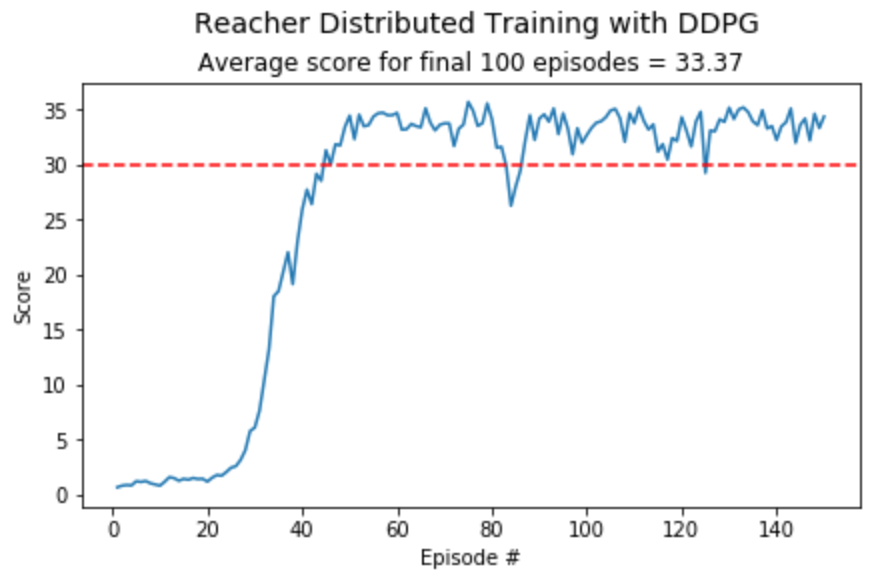
\includegraphics[width=3.0in]{ddpg-scores}
	\label{fig:ddpg-scores}
	\caption{Training Scores}
\end{figure}


\section{Improving Performance}

Deep Deterministic Policy Gradient did well on this task.  To improve performance futher, I would do grid search on the hyper-parameters and network architectures for this approach.  Another interesting direction would be to try the {\em Soft Actor-Critic Algorthm}~\cite{DBLP:journals/corr/abs-1812-05905}.  The key idea 
of this algorithm is to add an entropy constraint to the characterization of an optimal policy:
	$$\pi^* =  \operatorname{arg\,max}_{\pi}\mathbb{E}_{\tau\sim\pi}\big[\sum_{t=0}^{\infty}\gamma^t\big(R_t+\alpha \mathcal{H} [\pi(\cdot|S_t)]\big)\big],$$
which can result in more stable learning.

\bibliographystyle{ACM-Reference-Format}
%%\nocite{*}
\bibliography{report}


\end{document}

The specific policy-based method I'll used is called {\em Deep Deterministic Policy Gradient}~\cite{Silver:2014:DPG:3044805.3044850} (DDPG) which 
concurrently learns a policy and a Q-function. Recall that the {\em Q-function} for a policy $\pi$ is defined by
$$Q^{\pi}(s,a) = \mathbb{E}_\pi\big[G_t| S_t = s, A_t=a\big].$$
DDPG uses  off-policy data and the \textbf{Bellman Equation}:
$$Q^{\pi}(s,a) = \mathbb{E}_\pi\big[R_{t+1}+\gamma\cdot Q^{\pi}(S_{t+1},A_{t+1})| S_t = s, A_t=a\big].$$
to learn the Q-function, and uses the Q-function to learn the policy.

%%%%%%%%%%%%%%%%%%%%%%%%%%%%%%%%%%%%%%%%%%%%%%%%%%%%%%%%%%%%%%
%% Deep Q-Learning for Navigation                                                                                                %%
%%%%%%%%%%%%%%%%%%%%%%%%%%%%%%%%%%%%%%%%%%%%%%%%%%%%%%%%%%%%%%
\section{Soft Actor-Critic}

\subsection{Entropy-Regularized Reinforcement Learning}

$$\pi^* =  \operatorname{arg\,max}_{\pi}\mathbb{E}_{\tau\sim\pi}\big[\sum_{t=0}^{\infty}\gamma^t\big(R_t+\alpha \mathcal{H} [\pi(\cdot|S_t)]\big)\big].$$

$$L(\phi_i, {\mathcal D}) = \underset{(s,a,r,s',d) \sim {\mathcal D}}{\mathbb{E}}\left[
\Bigg( Q_{\phi_i}(s,a) - \left(r + \gamma (1 - d) V_{\psi_{\text{targ}}}(s') \right) \Bigg)^2
\right].$$

{\em Soft Actor-Critic Algorthm}~\cite{DBLP:journals/corr/abs-1812-05905}.
Source code in Python, using PyTorch, is available on 
\href{http://github.com}{\underline{github}} 
in the repo 
\href{https://github.com/bobflagg/Actor-Critic-for-Continuous-Control}{\underline{Actor-Critic-for-Continuous-Control}}.

For a policy $\pi$, the {\em state-value function}, $V^\pi$, is defined by
$$V^{\pi}(s) = \mathbb{E}_\pi\big[G_t| S_t = s\big].$$
and we would like to find $\pi$ so that 
$$V^{\pi}(s) = V^{*}(s) = \max_{\pi'}V^{\pi'}(s).$$



%%%%%%%%%%%%%%%%%%%%%%%%%%%%%%%%%%%%%%%%%%%%%%%%%%%%%%%%%%%%%%
%% Resources                                                                                                                               %%
%%%%%%%%%%%%%%%%%%%%%%%%%%%%%%%%%%%%%%%%%%%%%%%%%%%%%%%%%%%%%%
\section{Additional Resources}

\begin{enumerate}
	
	\item \href{https://blog.lateral.io/2017/10/text-segmentation-using-word-embeddings/}{\color{red}Text Segmentation using Word Embeddings}
	\item \href{http://www.cs.man.ac.uk/~mary/choif/software.html}{\color{red}Freddy Choi: Code and data for segmentation experiments}
	\item \href{https://github.com/datafordemocracy/topictiling}{\color{red}Repository that does topictiling on cable news}
	\item \href{https://github.com/logological/C99}{\color{red}C99, a domain-independent algorithm for linear text segmentation by Freddy Choi}
	\item \href{https://github.com/levy5674/text-tiling-demo}{\color{red}Demo of ntlk's TextTilingTokenizer}
	\item \href{http://politicaladarchive.org/data/}{\color{red}Political TV Ad Archive}
	\item \href{http://classif.ai/dataset/tv-news-channel-commercial-detection-dataset/}{\color{red}TV News Channel Commercial Detection Dataset}
	\item \href{http://github.com/alexalemi/segmentation}{\color{red}Alex Alemi: Code and data for segmentation experiments}
	
\end{enumerate}


